\documentclass[12pt]{article}
\usepackage[utf8]{inputenc}
\usepackage{amsmath}
\usepackage{graphicx}
\usepackage{geometry}
\usepackage{float}
\usepackage{caption}

\geometry{letterpaper, margin=1in}

\title{Homework 0}
\author{Naima Shariff}
\date{}

\begin{document}

\maketitle

\section*{Problem 1}

The first derivative of the function $f(x) = \exp(\sin(x))$ was computed on the interval $0 \le x \le 2\pi$.
The numerical approximation uses second-order centered finite differences for the internal grid points and first-order one-sided differences at the boundaries.

Figure \ref{fig:p1_comparison} shows the analytical solution plotted alongside the numerical approximation, as well as the absolute error between the two. Error is largest at the ends.

\begin{figure}[H]
    \centering
    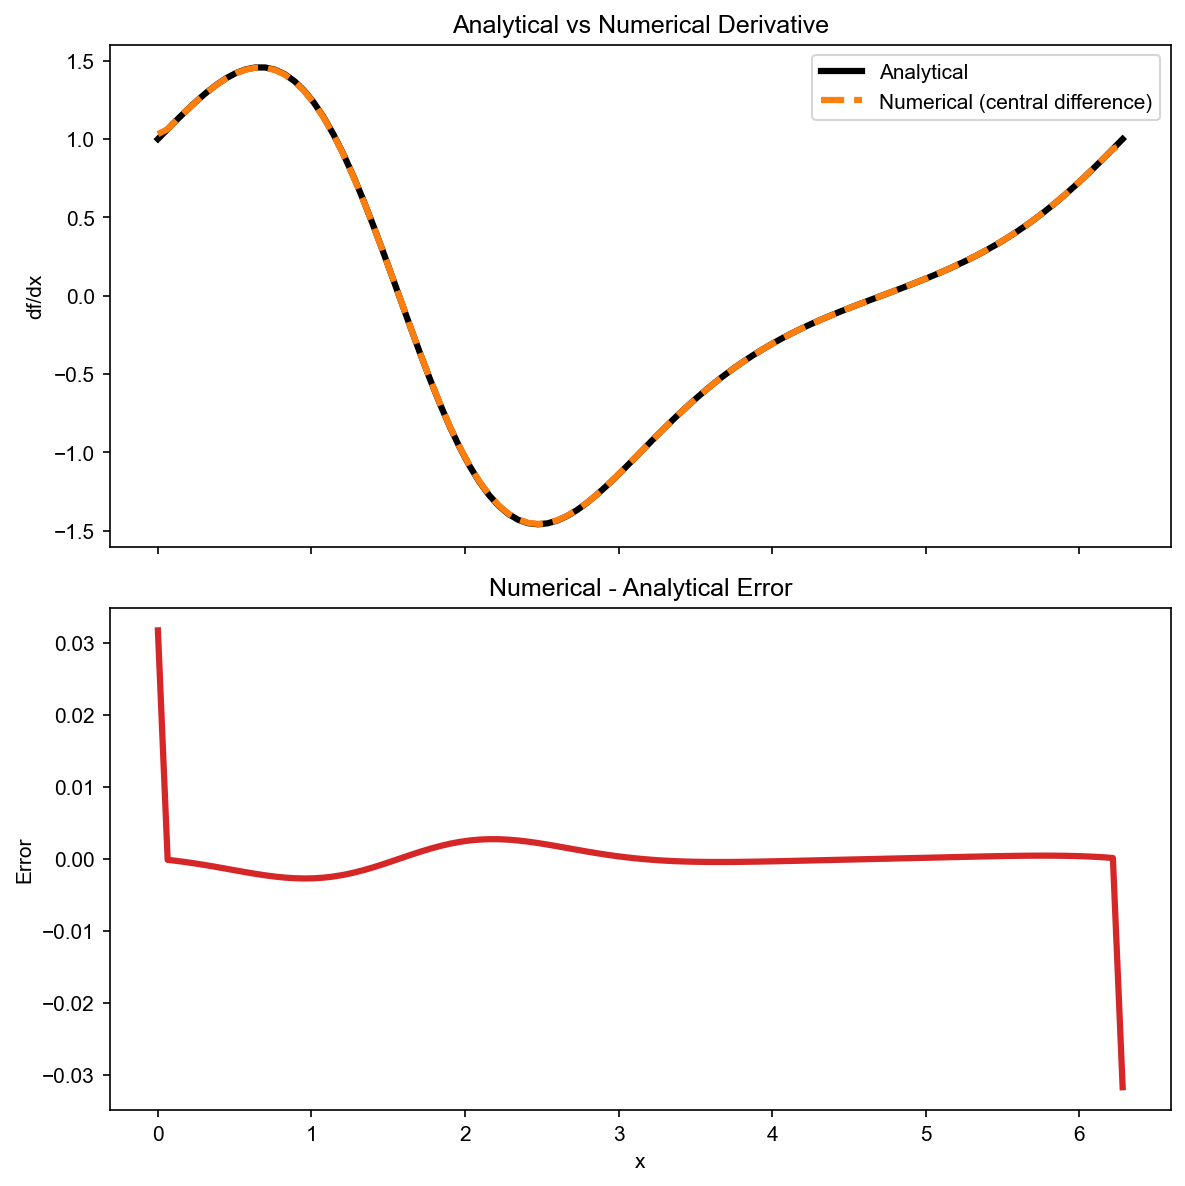
\includegraphics[width=0.8\textwidth]{figures/hw0_first_derivative_comparison.png}
    \caption{Comparison of analytical and numerical first derivatives of $f(x)$.}
    \label{fig:p1_comparison}
\end{figure}


Convergence plots for a range of $N$ values showed the relative error under the $L_\infty$ and $L_2$ norms against the grid size $N$ 

\begin{figure}[H]
    \centering
    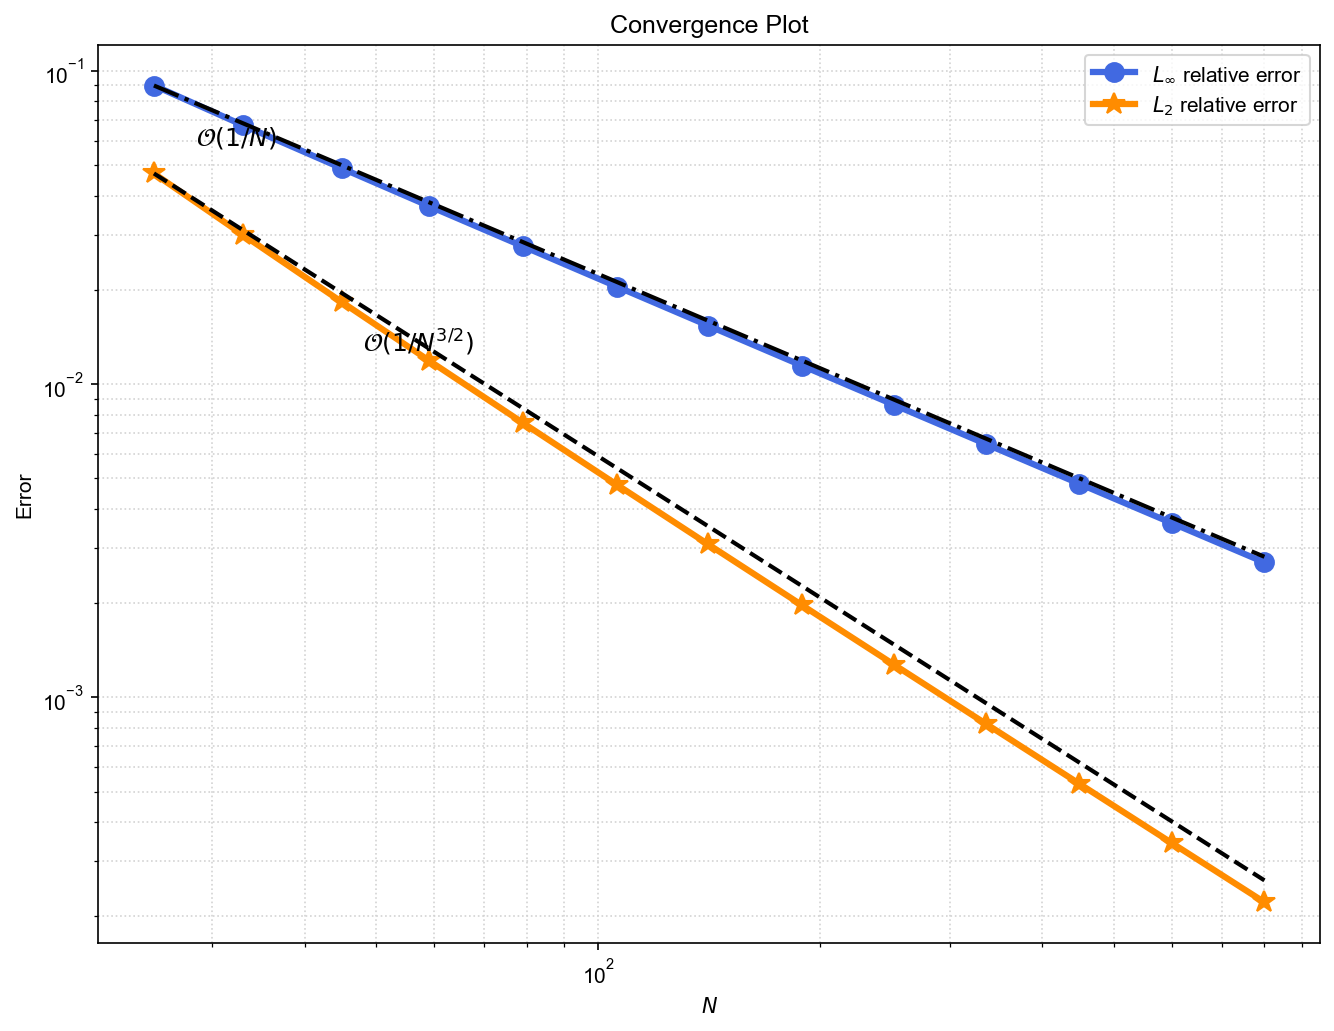
\includegraphics[width=0.8\textwidth]{figures/hw0_first_derivative_convergence.png}
    \caption{Relative error convergence using $L_\infty$ and $L_2$ norms.}
    \label{fig:p1_convergence}
\end{figure}

\subsection*{Extra Credit: The $3/2$ Slope for the $L_2$ Norm}

The convergence rates are obtained analytically by Taylor-expanding each finite-difference stencil about a grid point giving the error estimation at that point: $O(h^2)$ for the central-difference approximation used at interior nodes, and $O(h)$ for the one-sided approximation used at the two boundary nodes. $L_\infty$ norm reports only the single largest error in the domain, it is dominated entirely by the lower-order boundary stencil resulting in a global rate of $O(1/N)$. The $L_2$ relative error additionally normalizes by $|f'(x)|_2$, which grows as $O(N^{1/2})$ since it aggregates an increasing number of similarly-sized terms as the grid is refined; dividing the $O(1/N)$ error norm by this growing quantity yields the compounded rate $O(N^{-3/2})$.

The theoretical predictions are verified empirically by computing the local convergence rate between successive grid refinements, $p \approx \log(e_{i+1}/e_i)/\log(N_{i+1}/N_i)$, from the simulation data. The measured rates converged to approximately $-1$ and $-3/2$ for the $L_\infty$ and $L_2$ norms, respectively.

\section*{Problem 2}

The second derivative $f''(x)$ was computed using a second-order central difference with periodic boundary conditions.
Figure \ref{fig:p2_comparison} shows the comparison of analytical and numerical second derivatives of $f(x)$

\begin{figure}[H]
    \centering
    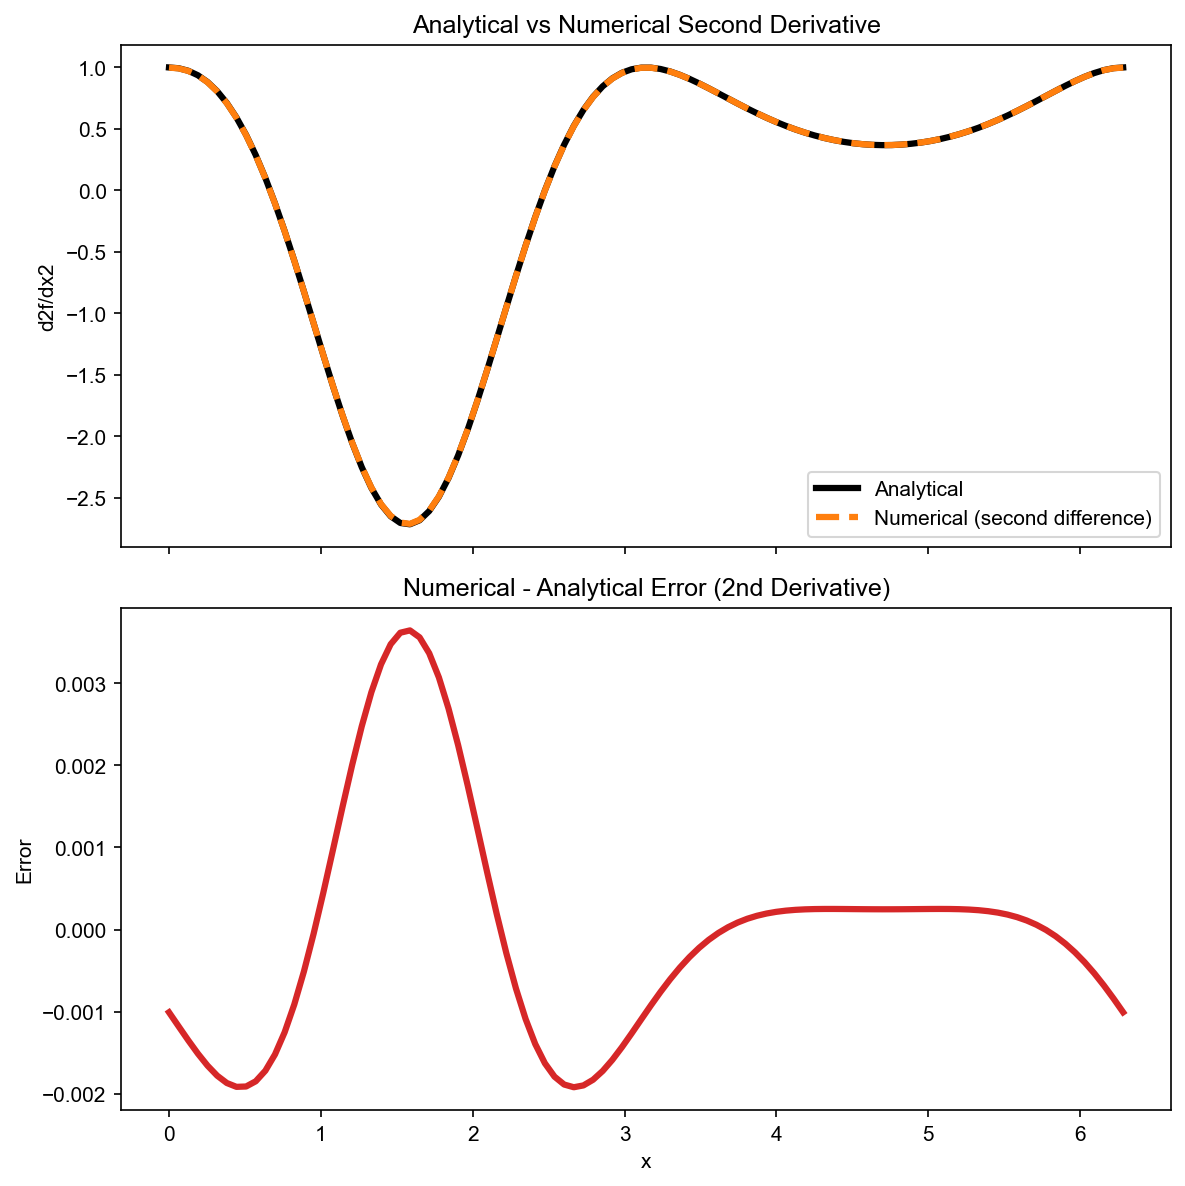
\includegraphics[width=0.8\textwidth]{figures/hw0_second_derivative_comparison.png}
    \caption{Comparison of analytical and numerical second derivatives of $f(x)$.}
    \label{fig:p2_comparison}
\end{figure}

Convergence plots for a range of $N$ values showed the relative error under the $L_\infty$ and $L_2$ norms against the grid size. The error scaling confirms the expected $\mathcal{O}(1/N^2)$ second-order convergence for both norms, as the periodic boundary conditions avoids the introduction of first-order boundary errors.

\begin{figure}[H]
    \centering
    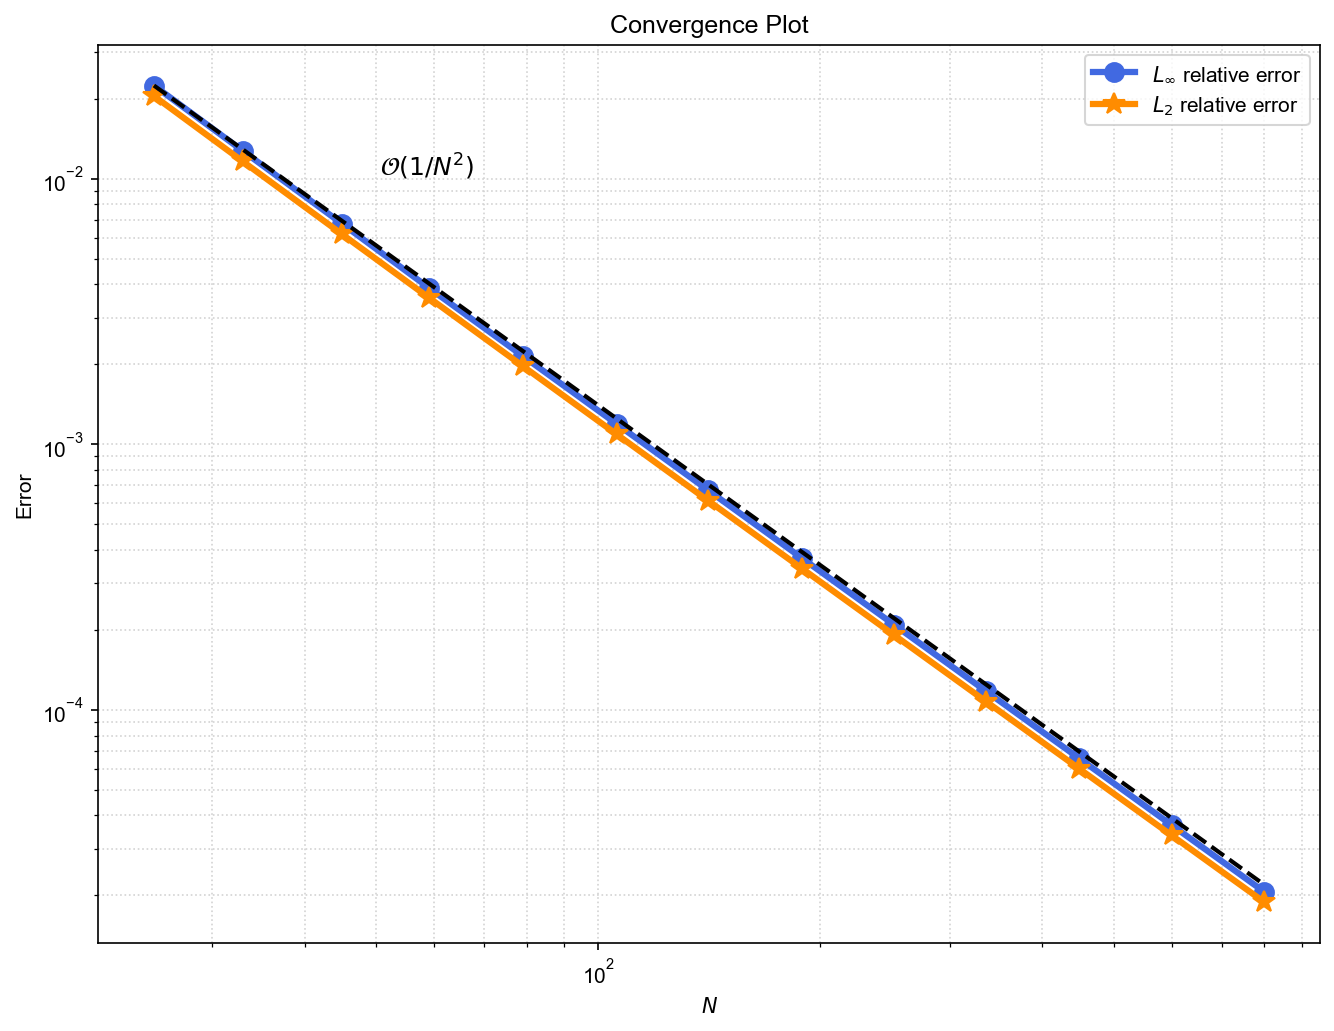
\includegraphics[width=0.8\textwidth]{figures/hw0_second_derivative_convergence.png} %[cite: 6]
    \caption{Relative error convergence confirming $\mathcal{O}(1/N^2)$ accuracy for the second derivative.}
    \label{fig:p2_convergence}
\end{figure}

\section*{Problem 3}

\begin{figure}[H]
    \centering
    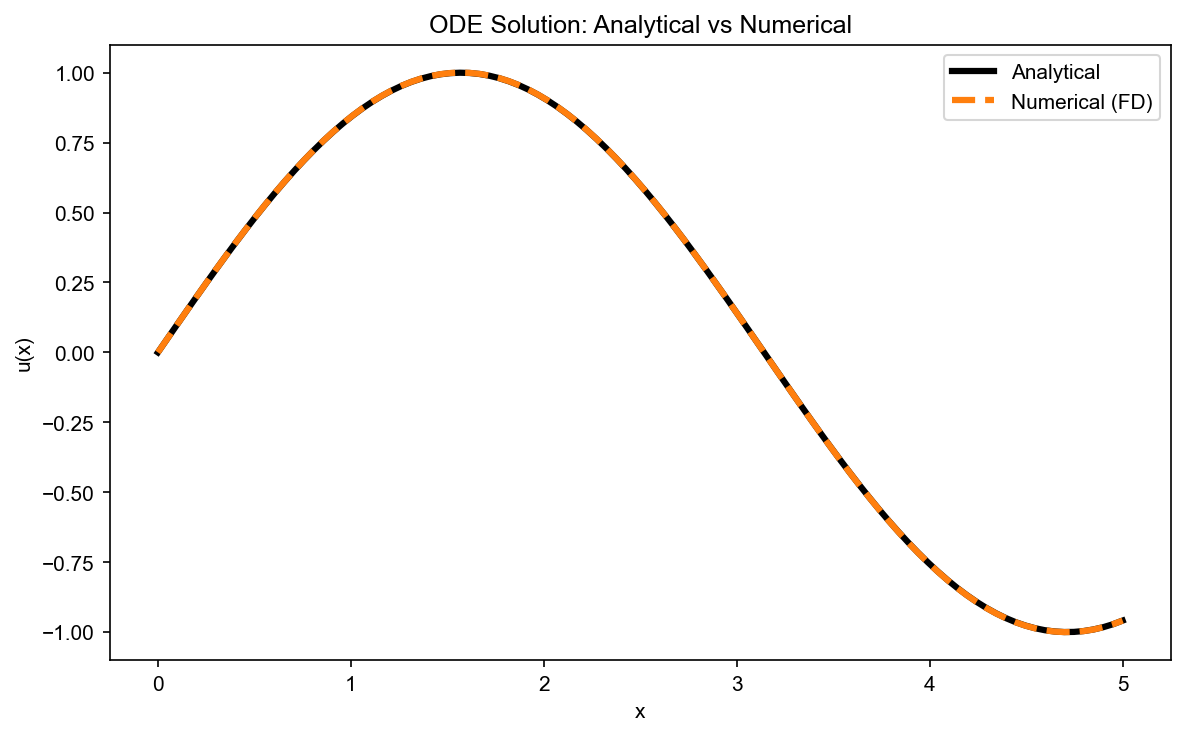
\includegraphics[width=0.8\textwidth]{figures/problem3_solution_comparison.png}
    \caption{Comparison of analytical and numerical solutions for the ODE.}
    \label{fig:p3_comparison}
\end{figure}

The tri-diagonal stencil was derived by substituting the second-order central-difference approximations $u'' \approx (u_{i+1} - 2u_i + u_{i-1})/h^2$ and $u' \approx (u_{i+1} - u_{i-1})/(2h)$ directly into the governing ODE, then collecting like terms in $u_{i-1}$, $u_i$, and $u_{i+1}$ to obtain the coefficients $a_i = 1/h^2 - \sin(x_i)/2h$, $b_i = -2/h^2 + 1$, and $c_i = 1/h^2 + \sin(x_i)/2h$. The resulting finite-difference solution is a good approximation of the analytical solution $u(x) = \sin(x)$ across the domain.

\begin{figure}[H]
    \centering
    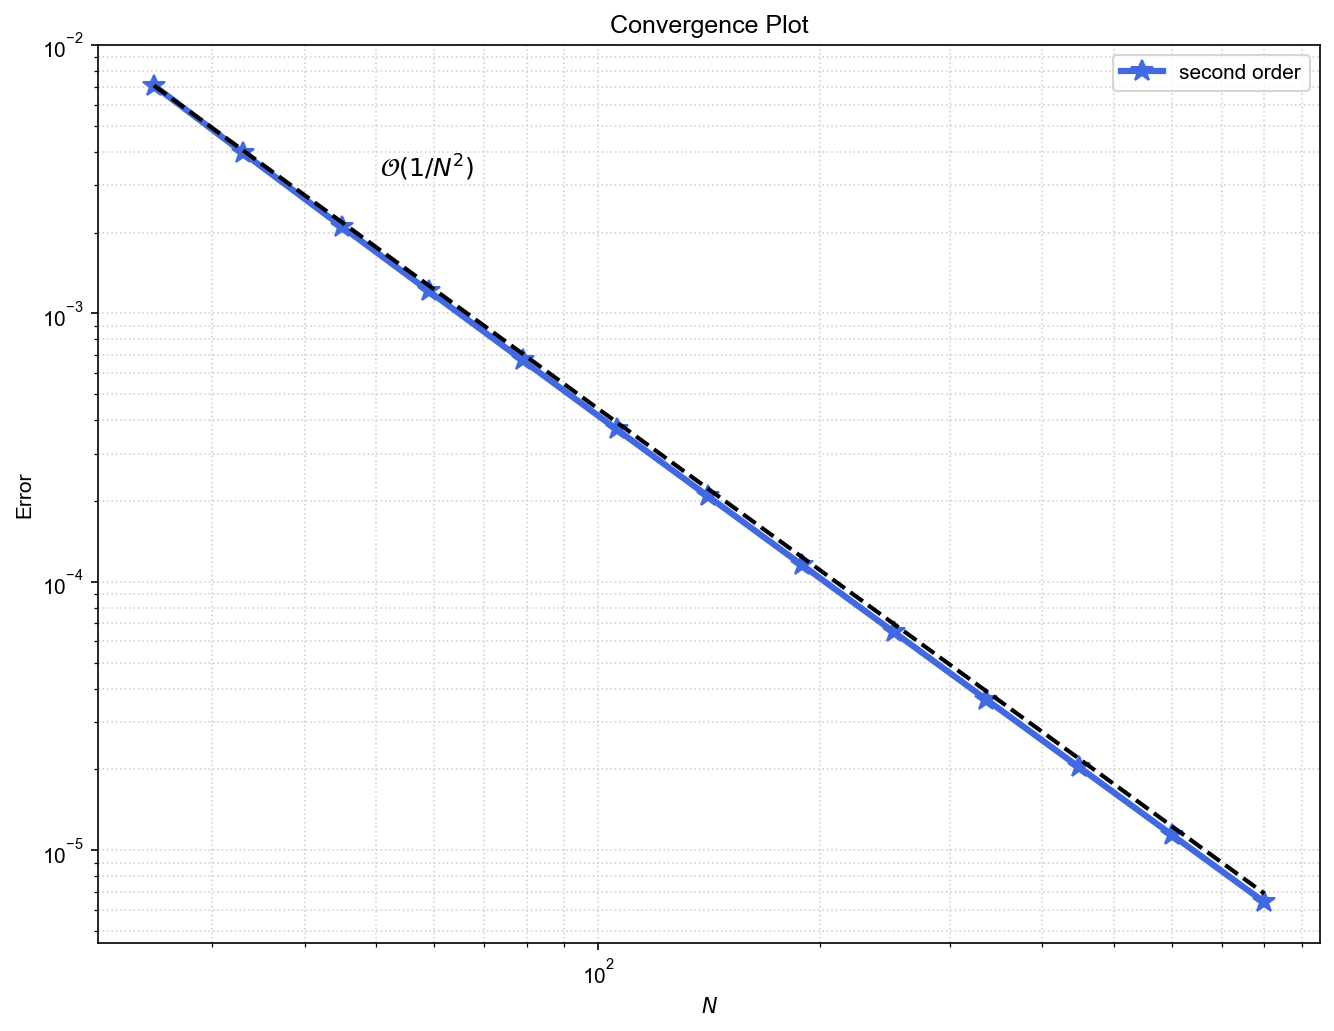
\includegraphics[width=0.8\textwidth]{figures/problem3_convergence.png} 
    \caption{Relative error convergence confirming second-order accuracy.}
    \label{fig:p3_convergence}
\end{figure}

The convergence plots for a range of $N$ values showed the relative $L_2$ error against the grid size $N$, showing a second-order convergence $\mathcal{O}(1/N^2)$ for the finite difference scheme implemented.

\section*{Problem 4}

The Poisson equation $\nabla^2 u = f(x,y)$ was solved over the two-dimensional domain $x \in [0, 5], y \in [0, 5]$ using a second-order finite difference method. Dirichlet boundary conditions were applied on all boundaries to satisfy the test solution $u(x,y) = \sin(x)\cos(y)$ 
The analytical derivation of the forcing function resulted in $f(x,y) = -2\sin(x)\cos(y)$
Figure \ref{fig:p4_comparison} displayed the analytical solution, the numerical finite difference approximation, and the numerical-analytical error distribution. 

\begin{figure}[H]
    \centering
    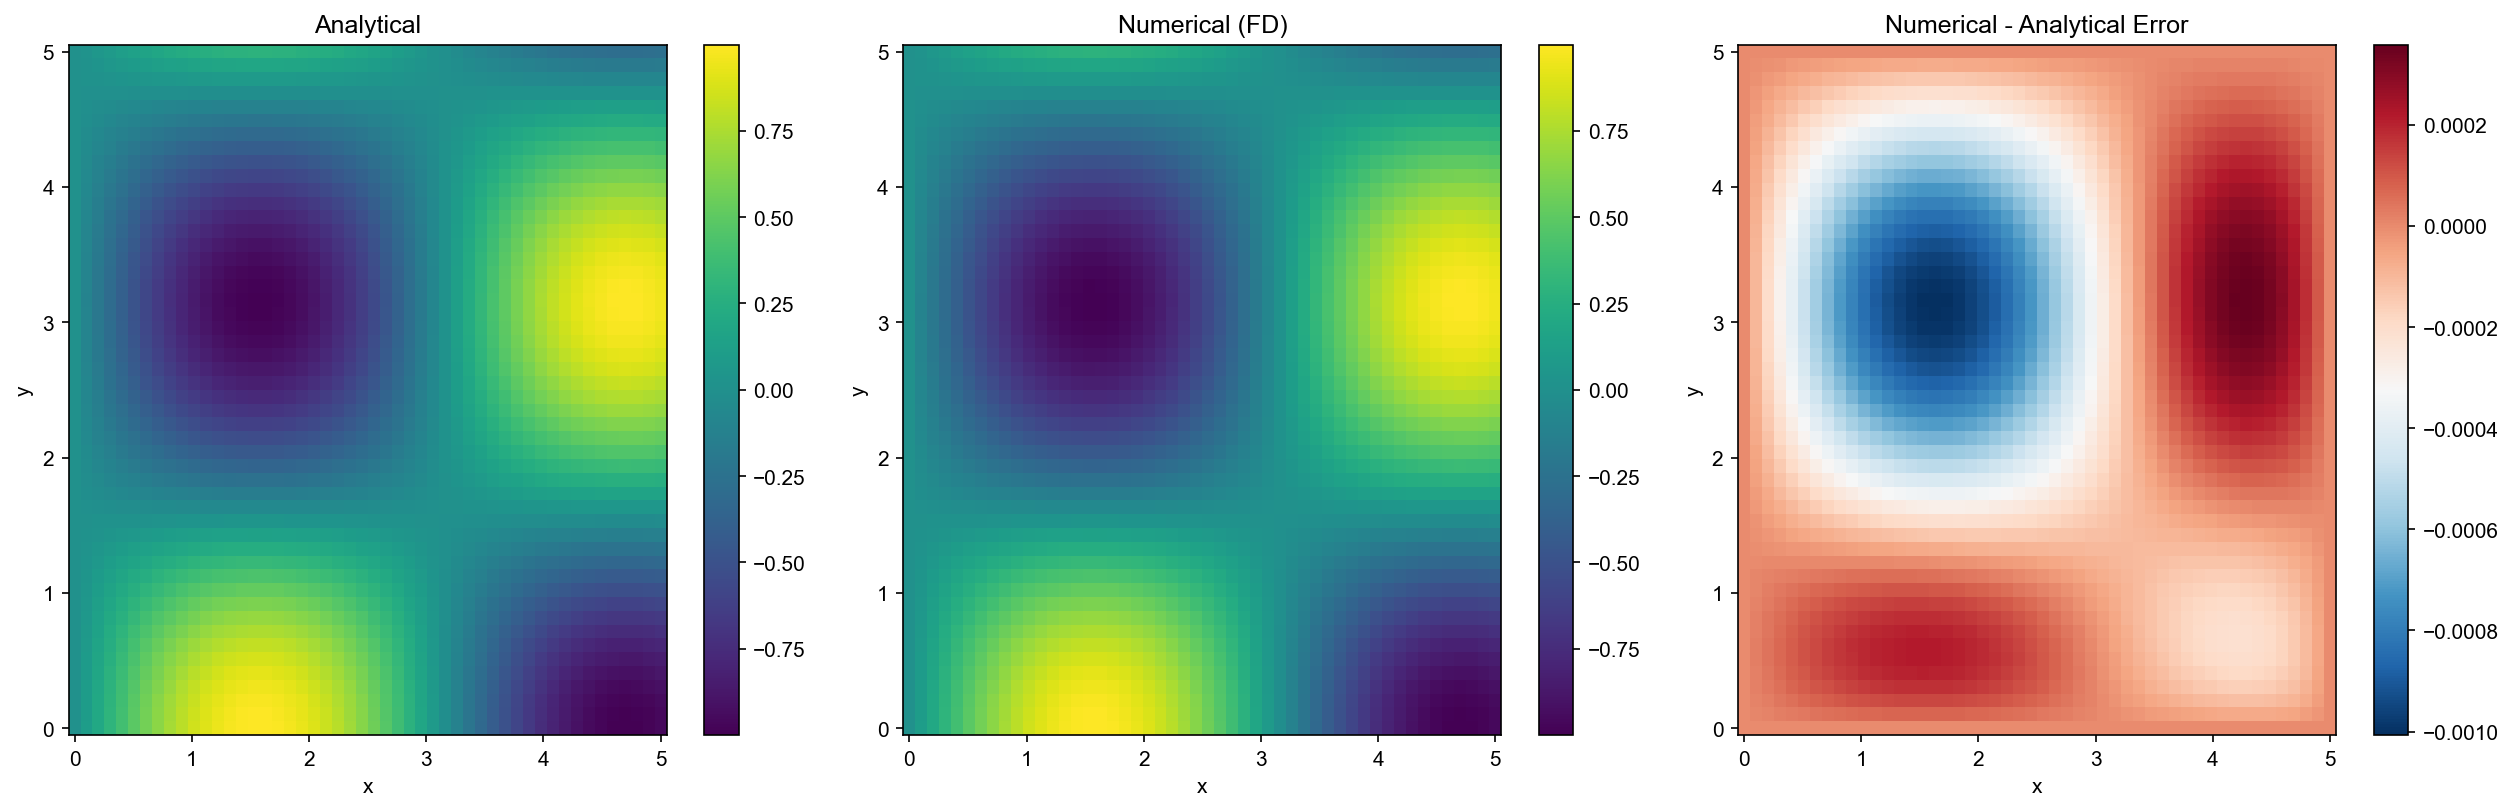
\includegraphics[width=1\textwidth]{figures/problem4_solution_comparison.png}
    \caption{Comparison of analytical and numerical solutions for the Poisson equation.}
    \label{fig:p4_comparison}
\end{figure}

The error-generating term is proportional to $u$ itself, so it's largest in magnitude where $u$ is largest in magnitude 

Convergence plots for a range of $N$ values showed the relative $L_2$ error scaling against the grid size $N$
The error scaling is $\mathcal{O}(1/N^2)$. 

\begin{figure}[H]
    \centering
    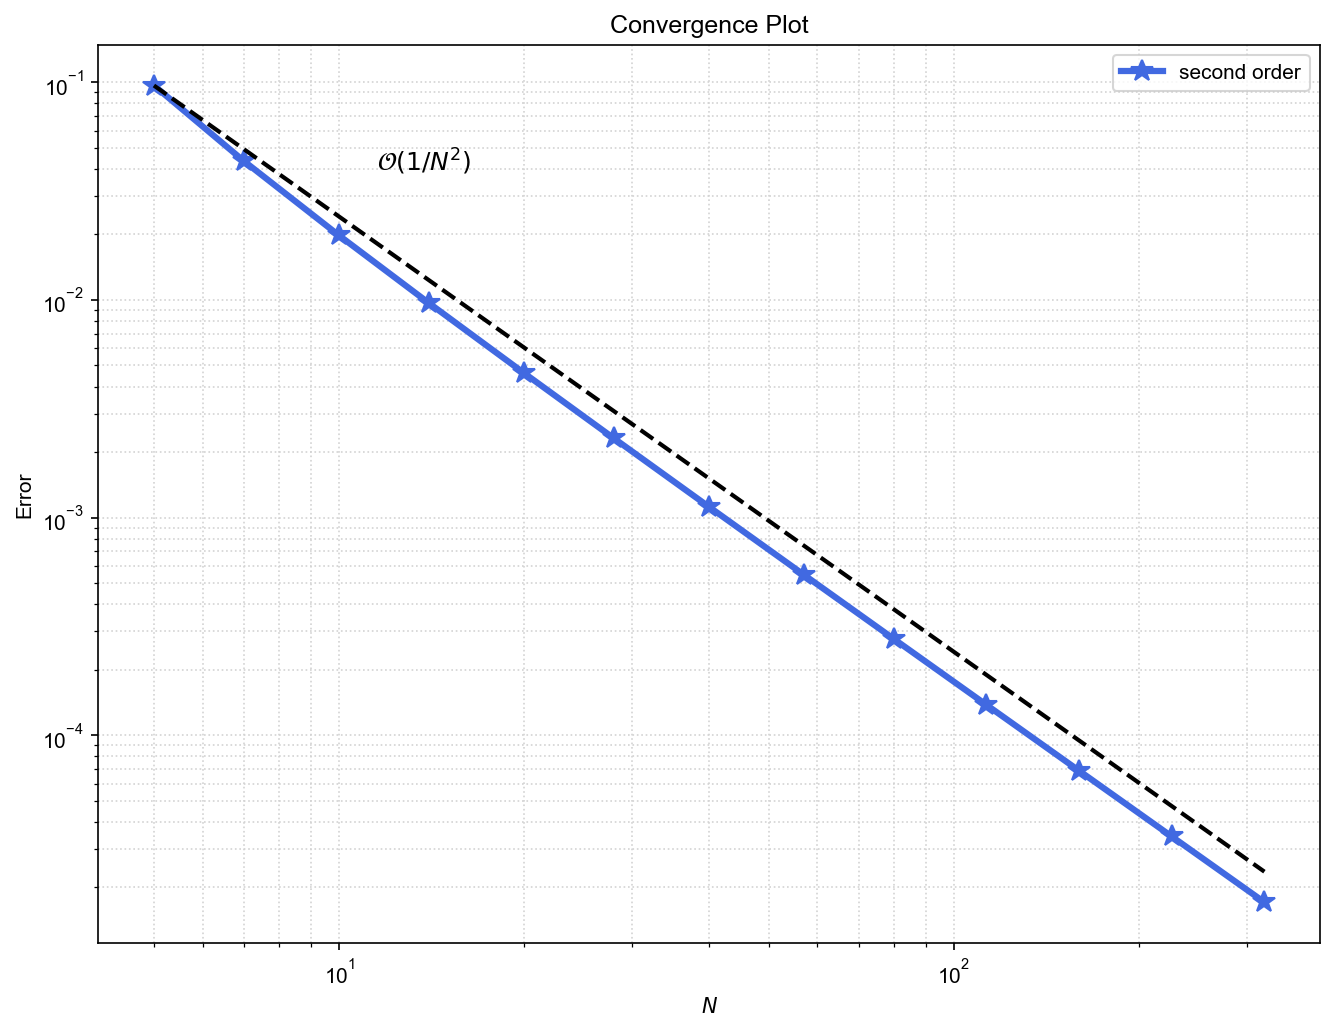
\includegraphics[width=0.8\textwidth]{figures/problem4_convergence.png}
    \caption{Relative error convergence(second-order accuracy for the Poisson equation).}
    \label{fig:p4_convergence}
\end{figure}

\subsection*{Why pure Neumann conditions fail}

Every row's coefficients sum to zero (interior: $1+1+1+1-4=0$; Neumann boundary: $\pm 1/h \mp 1/h = 0$), so the constant vector is exactly in the null space of $A$. The matrix is singular, confirmed numerically by $\max |A\mathbf{1}| = 0$. The solver does not raise an error on this; it silently returns an unreasonable solution with norm $\sim 10^{15}$. This matches the PDE itself: a pure-Neumann Poisson problem requires
\begin{equation}
    \int_\Omega f \, dA = \oint_{\partial\Omega} \frac{\partial u}{\partial n} \, ds
\end{equation}
to have a solution at all, and even then $u$ is only defined up to an arbitrary additive constant, exactly the null direction found above.

\textbf{Fix:} pin $u$ at one grid point (Dirichlet) to remove the null space. This only works if the pinned point is interior (or a non-corner boundary point), pinning a corner leaves the matrix rank-deficient by 1, as verified directly.

\textit{This explanation was developed with the assistance of Claude (Anthropic) Model: Sonnet(High).}


\section*{Acknowledgment}
All plotting routines used to generate the figures in this report were developed with the assistance of Claude (Sonnet 5), an AI model developed by Anthropic.

\end{document}


